\documentclass[crop,tikz,convert=pdf2svg,8pt]{standalone}

% Tikz settings optimized for causal graphs.
\usetikzlibrary{shapes,decorations,arrows,calc,arrows.meta,fit,positioning}
\tikzset{
    -Latex,auto,node distance =1 cm and 1 cm,semithick ,
    state/.style ={ellipse, draw, minimum width = 0.7 cm},
    point/.style = {circle, draw, inner sep=0.04cm,fill,node contents={}},
    bidirected/.style={Latex-Latex,dashed},
    el/.style = {inner sep=2pt, align=left, sloped}
}

\begin{document}

% The graph
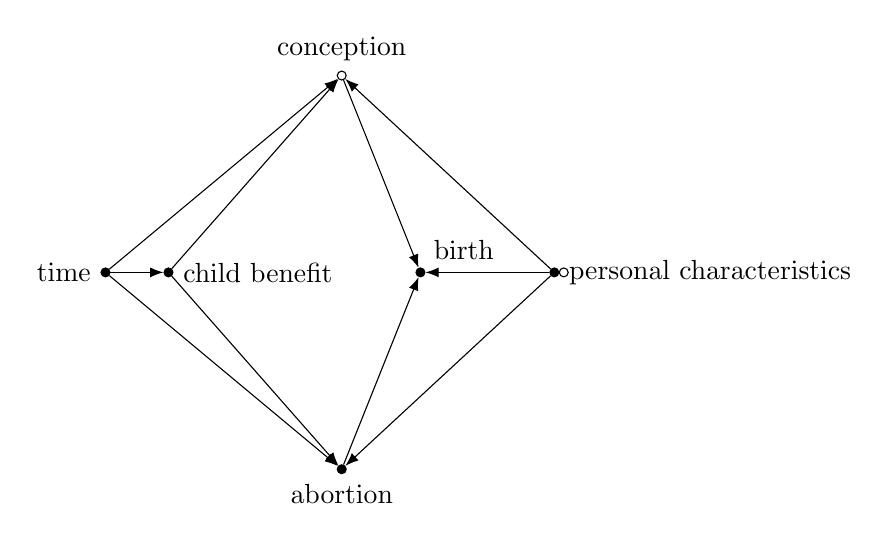
\begin{tikzpicture}
    \node (t) at (0,0) [label=left:time, point];
    \node (D) at (0.8,0) [label=right:child benefit, point];
    \node (c) at (3,2.5) [label=above:conception, point, fill=none];
    \node (a) at (3,-2.5) [label=below:abortion, point];
		\node (b) at (4,0) [label=above right:birth, point];
		\node (p) at (5.7,0) [label=right:personal characteristics, point];
		\node (pu) at (5.82,0) [point, fill=none];

    \path (t) edge (D);
		\path (t) edge (c);
		\path (t) edge (a);
    \path (D) edge (c);
		\path (D) edge (a);
		\path (c) edge (b);
		\path (a) edge (b);
		\path (p) edge (c);
		\path (p) edge (a);
		\path (p) edge (b);
    %\path[bidirected] (2) edge[bend left=50]  (3);
\end{tikzpicture}

\end{document}